\documentclass[12pt, titlepage]{article}

\usepackage{amsmath, mathtools}
\usepackage{amsfonts}
\usepackage{amssymb}
\usepackage{booktabs}
\usepackage{tabularx}
\usepackage{xspace}

\usepackage{graphicx}
\usepackage{colortbl}
\usepackage{xr}
\usepackage{longtable}
\usepackage{xfrac}
\usepackage{float}
\usepackage{siunitx}
\usepackage{caption}
\usepackage{pdflscape}
\usepackage{afterpage}

\usepackage{fullpage}
\usepackage[round]{natbib}
\usepackage{multirow}
%\usepackage{refcheck}
\usepackage{lipsum}

%% Comments

\usepackage{color}

\newif\ifcomments\commentsfalse

\ifcomments
\newcommand{\authornote}[3]{\textcolor{#1}{[#3 ---#2]}}
\newcommand{\todo}[1]{\textcolor{red}{[TODO: #1]}}
\else
\newcommand{\authornote}[3]{}
\newcommand{\todo}[1]{}
\fi

\newcommand{\wss}[1]{\authornote{blue}{SS}{#1}} 
\newcommand{\plt}[1]{\authornote{magenta}{TPLT}{#1}} %For explanation of the template
\newcommand{\an}[1]{\authornote{cyan}{Author}{#1}}
\newcommand{\jme}[1]{\authornote{cyan}{JME}{#1}}

% Common Parts

\usepackage{tabularx}
\usepackage{booktabs}
\usepackage{ifthen}
\usepackage{amsmath,amssymb,xspace}

%PUT YOUR PROGRAM NAME HERE %Every program should have a name
\newcommand{\progname}[1]
{%
  \ifthenelse{\equal{#1}{n}}{{\normalsize ROC\xspace}}{}%
  \ifthenelse{\equal{#1}{L}}{{\Large ROC\xspace}}{}%
  \ifthenelse{\equal{#1}{f}}{{\footnotesize ROC\xspace}}{}%
}
% Abbreviations
\newcommand{\ode}{{\footnotesize ODE}\xspace}
\newcommand{\dae}{{\footnotesize DAE}\xspace}
\newcommand{\ivp}{{\footnotesize IVP}\xspace}
\newcommand{\fadbad}{{\footnotesize FADBAD++}\xspace}
\newcommand{\plainc}{{\footnotesize C}\xspace}
\newcommand{\cpp}{{\footnotesize C++}\xspace}
\newcommand{\adolc}{{\footnotesize ADOL-C}\xspace}
\newcommand{\rdcon}{{\footnotesize DRDCV}\xspace}
\newcommand{\fortran}{{\footnotesize FORTRAN 77}\xspace}
\newcommand{\daets}{{\footnotesize DAETS}\xspace}
\newcommand{\matlab}{{\footnotesize MATLAB}\xspace}
\newcommand{\mathematica}{{\footnotesize MATHEMATICA}\xspace}
\newcommand{\maple}{{\footnotesize MAPLE}\xspace}
% User commands
\newcommand{\Quote}[1]{``{#1}''}
\newcommand{\Ni}{\noindent}
% Environment
\newcommand{\EQ}[1]{\begin{align} {#1} \end{align}}
% Mathematics
\newcommand{\parn}[1]{( {#1} )}
\newcommand{\parbg}[1]{\left(  {#1} \right)}
\newcommand{\pbg}[1]{\bigl(  {#1} \bigr)}
\newcommand{\Setbg}[1]{\bigl\{ {#1} \bigr\}}
\def\Rz{\mathbb{R}}
\def\Cz{\mathbb{C}}
\newcommand{\nliminf}[1]{\liminf\limits_{{#1} \rightarrow \infty}}
\newcommand{\nlimsup}[1]{\limsup\limits_{{#1} \rightarrow \infty}}
% Mathematics: ODE
\newcommand{\iode}{\protect{\makebox{$[t_0,\tend]$}}\xspace}
\newcommand{\lode}{\protect{\makebox{$[t_n,t_{n+1}]$}}\xspace}
\newcommand{\tend}{t_\text{end}}
\newcommand{\tc}[2]{(#1)_{#2}}
\newcommand{\Tp}{T}
\newcommand{\xn}{x_{n}}
\newcommand{\tn}{t_{n}}
% Reference
\renewcommand{\eqref}[1]{(\ref{eq:#1})}
\newcommand{\rrf}[2]{(\ref{eq:#1}--\ref{eq:#2})}
\newcommand{\chref}[1]{\ref{ch:#1}}
\newcommand{\sscref}[1]{\ref{ssc:#1}}
\newcommand{\scref}[1]{Section~\ref{sc:#1}}
\newcommand{\exref}[1]{\ref{ex:#1}}
\newcommand{\rmref}[1]{\ref{rm:#1}}
\newcommand{\apref}[1]{\ref{ap:#1}}
%\newcommand{\tbref}[1]{\ref{tb:#1}}
\newcommand{\dfref}[1]{\ref{df:#1}}
\newcommand{\leref}[1]{\ref{le:#1}}
\newcommand{\fgref}[1]{\ref{fg:#1}}
\newcommand{\coref}[1]{\ref{co:#1}}
\newcommand{\thref}[1]{\ref{th:#1}}
\newcommand{\agref}[1]{\ref{ag:#1}}
\newcommand{\asref}[1]{\ref{as:#1}}
\newcommand{\EQref}[1]{Equation~(\ref{eq:#1})}
\newcommand{\CHref}[1]{Chapter~\ref{ch:#1}}
\newcommand{\SSCref}[1]{Subsection~\ref{ssc:#1}}
\newcommand{\SCref}[1]{Section~\ref{sc:#1}}
\newcommand{\EXref}[1]{Example~\ref{ex:#1}}
\newcommand{\RMref}[1]{Remark~\ref{rm:#1}}
\newcommand{\APref}[1]{Appendix~\ref{ap:#1}}
\newcommand{\TBref}[1]{Table~\ref{tb:#1}}
\newcommand{\DFref}[1]{Definition~\ref{df:#1}}
\newcommand{\LEref}[1]{Lemma~\ref{le:#1}}
\newcommand{\FGref}[1]{Figure~\ref{fg:#1}}
\newcommand{\COref}[1]{Corollary~\ref{co:#1}}
\newcommand{\THref}[1]{Theorem~\ref{th:#1}}
\newcommand{\AGref}[1]{Algorithm~\ref{ag:#1}}
\newcommand{\ASref}[1]{Assumption~\ref{as:#1}}



\newcounter{acnum}
\newcommand{\actheacnum}{AC\theacnum}
\newcommand{\acref}[1]{AC\ref{#1}}
\newcommand{\aclabel}[1]{\refstepcounter{acnum} \actheacnum \label{#1}:}

\newcounter{ucnum}
\newcommand{\uctheucnum}{UC\theucnum}
\newcommand{\uref}[1]{UC\ref{#1}}
\newcommand{\uclabel}[1]{\refstepcounter{ucnum} \uctheucnum \label{#1}:}

\newcounter{mnum}
\newcommand{\mthemnum}{M\themnum}
\newcommand{\mref}[1]{M\ref{#1}}
\newcommand{\mlabel}[1]{\refstepcounter{mnum} \mthemnum \label{#1}:}

\begin{document}

\title{Module Guide for \progname{L}} 
\author{John M Ernsthausen}
\date{\today}

\maketitle

\pagenumbering{roman}

\section{Revision History}

\begin{tabularx}{\textwidth}{p{3.5cm}p{2cm}X}
\toprule {\bf Date} & {\bf Version} & {\bf Notes}\\
\midrule
  22 November 2020 & 1.0 & First submission\\
  04 December 2020 & 1.1 & First submission (before review)\\
\bottomrule
\end{tabularx}

\newpage

\section{Reference Material}

This section records information for easy reference.

\subsection{Abbreviations and Acronyms}

\renewcommand{\arraystretch}{1.2}
\begin{tabular}{l l} 
  \toprule		
  \textbf{symbol} & \textbf{description}\\
  \midrule 
  AC & Anticipated Change\\
  LC & Likely change\\
  M & Module \\
  MG & Module Guide \\
  OS & Operating System \\
  R & Requirement\\
  SC & Scientific Computing \\
  SRS & Software Requirements Specification\\
  \progname{f} & Radius of Convergence software developed for this project\\
  UC & Unlikely Change\\
  \bottomrule
\end{tabular}\\

\newpage

\tableofcontents

\listoftables

\listoffigures

\newpage

\pagenumbering{arabic}

\section{Introduction}

This document follows the MG Template for our course CSE 741, Development
of Scientific Computing Software, taught in the Fall of 2020 by Prof. Spencer Smith.
We are permitted to freely use the content of the MG Template.

Decomposing a system into modules is a commonly accepted approach to developing
software.  A module is a work assignment for a programmer or programming
team~\citep{ParnasEtAl1984}.  We advocate a decomposition
based on the principle of information hiding~\citep{Parnas1972a}.  This
principle supports design for change, because the ``secrets'' that each module
hides represent likely future changes.  Design for change is valuable in SC,
where modifications are frequent, especially during initial development as the
solution space is explored.  

Our design follows the rules laid out by \citet{ParnasEtAl1984}, as follows:
\begin{itemize}
\item System details that are likely to change independently should be the
  secrets of separate modules.
\item Each data structure is implemented in only one module.
\item Any other program that requires information stored in a module's data
  structures must obtain it by calling access programs belonging to that module.
\end{itemize}

After completing the first stage of the design, the Software Requirements
Specification (SRS), the Module Guide (MG) is developed~\citep{ParnasEtAl1984}. The MG
specifies the modular structure of the system and is intended to allow both
designers and maintainers to easily identify the parts of the software.  The
potential readers of this document are as follows:

\begin{itemize}
\item New project members: This document can be a guide for a new project member
  to easily understand the overall structure and quickly find the
  relevant modules they are searching for.
\item Maintainers: The hierarchical structure of the module guide improves the
  maintainers' understanding when they need to make changes to the system. It is
  important for a maintainer to update the relevant sections of the document
  after changes have been made.
\item Designers: Once the module guide has been written, it can be used to
  check for consistency, feasibility and flexibility. Designers can verify the
  system in various ways, such as consistency among modules, feasibility of the
  decomposition, and flexibility of the design.
\end{itemize}

The rest of the document is organized as follows. Section
\ref{SecChange} lists the anticipated and unlikely changes of the software
requirements. Section \ref{SecMH} summarizes the module decomposition that
was constructed according to the likely changes. Section \ref{SecConnection}
specifies the connections between the software requirements and the
modules. Section \ref{SecMD} gives a detailed description of the
modules. Section \ref{SecTM} includes two traceability matrices. One checks
the completeness of the design against the requirements provided in the SRS. The
other shows the relation between anticipated changes and the modules. Section
\ref{SecUse} describes the use relation between modules.

\section{Anticipated and Unlikely Changes} \label{SecChange}

This section lists possible changes to the system. According to the likeliness
of the change, the possible changes are classified into two
categories. Anticipated changes are listed in Section \ref{SecAchange}, and
unlikely changes are listed in Section \ref{SecUchange}.

\subsection{Anticipated Changes} \label{SecAchange}

Anticipated changes are the source of the information that is to be hidden
inside the modules. Ideally, changing one of the anticipated changes will only
require changing the one module that hides the associated decision. The approach
adapted here is called design for change. Anticipated changes are labeled by
{\bf AC} followed by a number.

\begin{description}
  \item[\aclabel{acIN}] The implementation of the input data structure.
    % Format and type of coefficients.
    % First coefficient corresponds to c_0, the coefficient of the zero power term,
    % to c_N, the coefficient of the N-1 power term. All real doubles. Scaling is real double.
  \item[\aclabel{acOUT}] The implementation of the output data structure.
    % Format and type of the radius of convergence R_c, order of singularity \mu, error in tail,
    % and error from coefficient MINTERMS to coefficient N-1.
  \item[\aclabel{acPARAM}] The implementation of the parameter data structure.
    % Format and type of parameters, distribution and constraints.
  \item[\aclabel{acSOLVER}] The algorithm used to solve the minimization sub-problem
    in 3TA, 6TA, and TLA.
  \item[\aclabel{acPoleRealSolver}] The algorithm used to find the distance to the
    nearest real pole.
  \item[\aclabel{acPoleComplexSolver}] The algorithm used to find the distance to
    the nearest complex conjugate pair of poles.
  \item[\aclabel{acPoleTopLine}] The algorithm used to find the distance to the nearest pole
    in top line analysis.
  \item[\aclabel{acROC}] How the overall control of the calculations is orchestrated.
    % Pole identification, distinguish a real pole from a complex conjugate pair of poles
    % from a complicated situation.
\end{description}

\subsection{Unlikely Changes} \label{SecUchange}

The module design should be as general as possible. However, a general system is
more complex. Sometimes this complexity is not necessary. Fixing some design
decisions at the system architecture stage can simplify the software design. If
these decision should later need to be changed, then many parts of the design
will potentially need to be modified. Hence, it is not intended that these
decisions will be changed. Unlikely changes are labeled by {\bf UC} followed by a number.

\begin{description}
  \item[\uclabel{ucHardware}] The hardware architecture is assumed to be a common personal
    computer running Ubuntu 20.04 or Windows 2010. The author does not have access
    to a personal computer running Mac OS, so Mac OS is excluded as well. However, the codes
    should not be written to exclude the Mac OS hardware architecture.
    We are not writing for graphic card architectures or other high performance computing clusters. 

  \item[\uclabel{ucAnalytic}] We assume that the inputs do not represent entire functions
    such as the exponential function.
\end{description}

\section{Module Hierarchy} \label{SecMH}

This section provides an overview of the module design. Modules are summarized
in a hierarchy decomposed by secrets in \TBref{module}. The modules listed
below, which are leaves in the hierarchy tree, are the modules that will
actually be implemented. Modules are labeled by {\bf M} followed by a number.


\begin{description}
  \item[\mlabel{mIN}] IN module.
  \item[\mlabel{mOUT}] OUT module.
  \item[\mlabel{mPARAM}] PARAM module.
  \item[\mlabel{mSOLVER}] SOLVER module.
  \item[\mlabel{mPoleRealSolver}] Real Pole module.
  \item[\mlabel{mPoleComplexSolver}] Complex Pair Poles module.
  \item[\mlabel{mPoleTopLineSolver}] Top Line Analysis module.
  \item[\mlabel{mROC}] ROC module.
\end{description}


\begin{table}[h!]
\centering
\begin{tabular}{p{0.3\textwidth} p{0.6\textwidth}}
\toprule
\textbf{Level 1} & \textbf{Level 2}\\
\midrule

\multirow{2}{0.3\textwidth}{Hardware-Hiding Module}
  & Input Format Module\\
  & Output Format Module \\

\midrule

\multirow{7}{0.3\textwidth}{Behaviour-Hiding Module}
  & Input Format Module\\
  & Output Format Module \\
  & Parameters Module\\
  & Real pole module\\
  & Complex conjugate pair of poles module\\ 
  & Resolve nearest pole in hard to resolve case module\\
  & Pole identification module\\
\midrule

{Software Decision Module} & Solver Module\\
\bottomrule

\end{tabular}
\caption{Module Hierarchy}
\label{tb:module}
\end{table}

\section{Connection Between Requirements and Design} \label{SecConnection}

The design of the system is intended to satisfy the requirements developed in
the SRS. In this stage, the system is decomposed into modules. The connection
between requirements and modules is listed in \TBref{TblRT}.

\wss{The intention of this section is to document decisions that are made
  ``between'' the requirements and the design.  To satisfy some requirements,
  design decisions need to be made.  Rather than make these decisions implicit,
  they are explicitly recorded here.  For instance, if a program has security
  requirements, a specific design decision may be made to satisfy those
  requirements with a password.  In scientific examples, the choice of algorithm
could potentially go here, if that is a decision that is exposed by the
interface.}

\section{Module Decomposition} \label{SecMD}

Modules are decomposed according to the principle of ``information hiding''
proposed by \citet{ParnasEtAl1984}. The \emph{Secrets} field in a module
decomposition is a brief statement of the design decision hidden by the
module. The \emph{Services} field specifies \emph{what} the module will do
without documenting \emph{how} to do it. For each module, a suggestion for the
implementing software is given under the \emph{Implemented By} title. If the
entry is \emph{OS}, this means that the module is provided by the operating
system or by standard programming language libraries.  \emph{\progname{f}} means the
module will be implemented by the \progname{f} software.

Only the leaf modules in the hierarchy have to be implemented. If a dash
(\emph{--}) is shown, this means that the module is not a leaf and will not have
to be implemented.

\subsection{Hardware Hiding Modules}

\subsubsection{Input Format Module (\mref{mIN})}

\begin{description}
\item[Secrets:] Handle input acquisition via hardware.
\item[Services:] Read files from hard drive.
  This module provides the interface between the hardware and the
  software. So, the system can use it to accept inputs.
\item[Implemented By:] OS
\end{description}

\subsubsection{Output Format Module (\mref{mOUT})}

\begin{description}
\item[Secrets:] Handle output via hardware.
\item[Services:] Write files to hard drive.
  This module provides the interface between the hardware and the
  software. So, the system can use it to display and save outputs.
\item[Implemented By:] OS
\end{description}

\subsection{Behaviour-Hiding Module}

\subsubsection{Input Format Module (\mref{mIN})}

\begin{description}
\item[Secrets:] The format and structure of the input data.
\item[Services:] Validate input format. Validate input type. Handle input acquisition via software.
\item[Implemented By:] \progname{f}
\item[Type of Module:] Library
\end{description}

\subsubsection{Output Format Module (\mref{mOUT})}

\begin{description}
\item[Secrets:] The format and structure of the output.
\item[Services:] Handle output format. Handle output type. Handle output via software.
\item[Implemented By:] \progname{f}
\item[Type of Module:] Library
\end{description}

\subsubsection{Parameters Module (\mref{mPARAM})}

\begin{description}
\item[Secrets:] Handle all aspects of parameters.
\item[Services:] This module handles parameter acquisition, format, type, distribution, and constraints.
\item[Implemented By:] \progname{f}
\item[Type of Module:] Record
\end{description}

\subsubsection{Real pole module (\mref{mPoleRealSolver})}

\begin{description}
\item[Secrets:] Implements solver for real poles.
\item[Services:] Computes $R_c$ and $\mu$ for real poles.
\item[Implemented By:] \progname{f}
\item[Type of Module:] Library
\end{description}

\subsubsection{Complex conjugate pair of poles module (\mref{mPoleComplexSolver})}

\begin{description}
\item[Secrets:] Implements solver for complex conjugate pair of poles.
\item[Services:] Computes $R_c$ and $\mu$ for complex conjugate pair of poles.
\item[Implemented By:] \progname{f}
\item[Type of Module:] Library
\end{description}

\subsubsection{Resolve nearest pole in hard to resolve case module (\mref{mPoleTopLineSolver})}

\begin{description}
\item[Secrets:] Implements solver to find the distance to the nearest pole in hard to resolve case.
\item[Services:] Computes $R_c$ for hard to resolve case.
\item[Implemented By:] \progname{f}
\item[Type of Module:] Library
\end{description}

\subsubsection{Pole identification module (\mref{mROC})}

\begin{description}
\item[Secrets:] Implements pole identification that distinguishes a real pole from
  a complex conjugate pair of poles from a complicated situation.
\item[Services:] Decides which solver is best suited to resolve the inputs.
\item[Implemented By:] \progname{f}
\item[Type of Module:] Library
\end{description}

\subsection{Software Decision Module (\mref{mSOLVER})}

\begin{description}
\item[Secrets:] Algorithms.
\item[Services:] Includes data structure and algorithms used in the system that
  do not provide direct interaction with the user.
  Algorithm to find the distance to the nearest real pole.
  Algorithm to find the distance to the nearest complex conjugate pair of poles.
  Algorithm to find the distance to the nearest pole in hard to resolve case.
  % Changes in these modules are more likely to be motivated by a desire to
  % improve performance than by externally imposed changes.
\item[Implemented By:] \progname{f}
\item[Type of Module:] Library
\end{description}

\section{Traceability Matrix} \label{SecTM}

This section shows two traceability matrices: between the modules and the
requirements and between the modules and the anticipated changes.

% the table should use mref, the requirements should be named, use something
% like fref
\begin{table}[H]
\centering
\begin{tabular}{p{0.2\textwidth} p{0.6\textwidth}}
\toprule
\textbf{Req.} & \textbf{Modules}\\
\midrule
  R1  & \mref{mIN}\\
  R2  & \mref{mIN}\\
  R3  & \mref{mIN}\\
  R4  & \mref{mIN}\\
  R5  & \mref{mIN}\\
  R6  & \mref{mIN}\\
  R7  & \mref{mOUT}\\
  R8  & \mref{mOUT}\\
  R9  & \mref{mOUT}\\
  R10 & \mref{mOUT}\\
  R11 & \mref{mPARAM}\\
  R12 & \mref{mPARAM}\\
  R13 & \mref{mPARAM}\\
  R14 & \mref{mPARAM}\\
  R15 & \mref{mPARAM}\\
  R16 & \mref{mSOLVER}\\
  R17 & \mref{mSOLVER}\\
  R18 & \mref{mSOLVER}\\
  R19 & \mref{mIN}, \mref{mOUT}, \mref{mPARAM}, \mref{mSOLVER}, \mref{mPoleRealSolver}, \mref{mROC}\\
  R20 & \mref{mIN}, \mref{mOUT}, \mref{mPARAM}, \mref{mSOLVER}, \mref{mPoleComplexSolver}, \mref{mROC}\\
  R21 & \mref{mIN}, \mref{mOUT}, \mref{mPARAM}, \mref{mSOLVER}, \mref{mPoleTopLineSolver}, \mref{mROC}\\
  R22 & \mref{mIN}, \mref{mOUT}, \mref{mROC}\\
  R23 & \mref{mIN}, \mref{mOUT},\mref{mPARAM}, \mref{mSOLVER}, \mref{mPoleRealSolver}, \mref{mPoleComplexSolver}, \mref{mPoleTopLineSolver}, \mref{mROC}\\
  R24 & \mref{mIN}, \mref{mOUT}, \mref{mPARAM}, \mref{mSOLVER}, \mref{mPoleRealSolver}, \mref{mROC}\\
  R25 & \mref{mIN}, \mref{mOUT}, \mref{mPARAM}, \mref{mSOLVER}, \mref{mPoleComplexSolver}, \mref{mROC}\\
  R26 & \mref{mIN}, \mref{mOUT}, \mref{mPARAM}, \mref{mSOLVER}, \mref{mPoleTopLineSolver}, \mref{mROC}\\
  R27 & \mref{mSOLVER}\\
\bottomrule
\end{tabular}
\caption{Trace Between Requirements and Modules}
\label{tb:TblRT}
\end{table}

\begin{table}[H]
\centering
\begin{tabular}{p{0.2\textwidth} p{0.6\textwidth}}
\toprule
\textbf{AC} & \textbf{Modules}\\
\midrule
  \acref{acIN} & \mref{mIN}\\
  \acref{acOUT} & \mref{mOUT}\\
  \acref{acPARAM} & \mref{mPARAM}\\
  \acref{acSOLVER} & \mref{mSOLVER}\\
  \acref{acPoleRealSolver} & \mref{mPoleRealSolver}\\
  \acref{acPoleComplexSolver} & \mref{mPoleComplexSolver}\\
  \acref{acPoleTopLine} & \mref{mPoleTopLineSolver}\\
  \acref{acROC} & \mref{mROC}\\
\bottomrule
\end{tabular}
\caption{Trace Between Anticipated Changes and Modules}
\label{TblACT}
\end{table}

\section{Use Hierarchy Between Modules} \label{SecUse}

In this section, the uses hierarchy between modules is
provided. \citet{Parnas1978} said of two programs A and B that A {\em uses} B if
correct execution of B may be necessary for A to complete the task described in
its specification. That is, A {\em uses} B if there exist situations in which
the correct functioning of A depends upon the availability of a correct
implementation of B.  Figure \ref{FigUH} illustrates the use relation between
the modules. It can be seen that the graph is a directed acyclic graph
(DAG). Each level of the hierarchy offers a testable and usable subset of the
system, and modules in the higher level of the hierarchy are essentially simpler
because they use modules from the lower levels.

\begin{figure}[H]
\centering
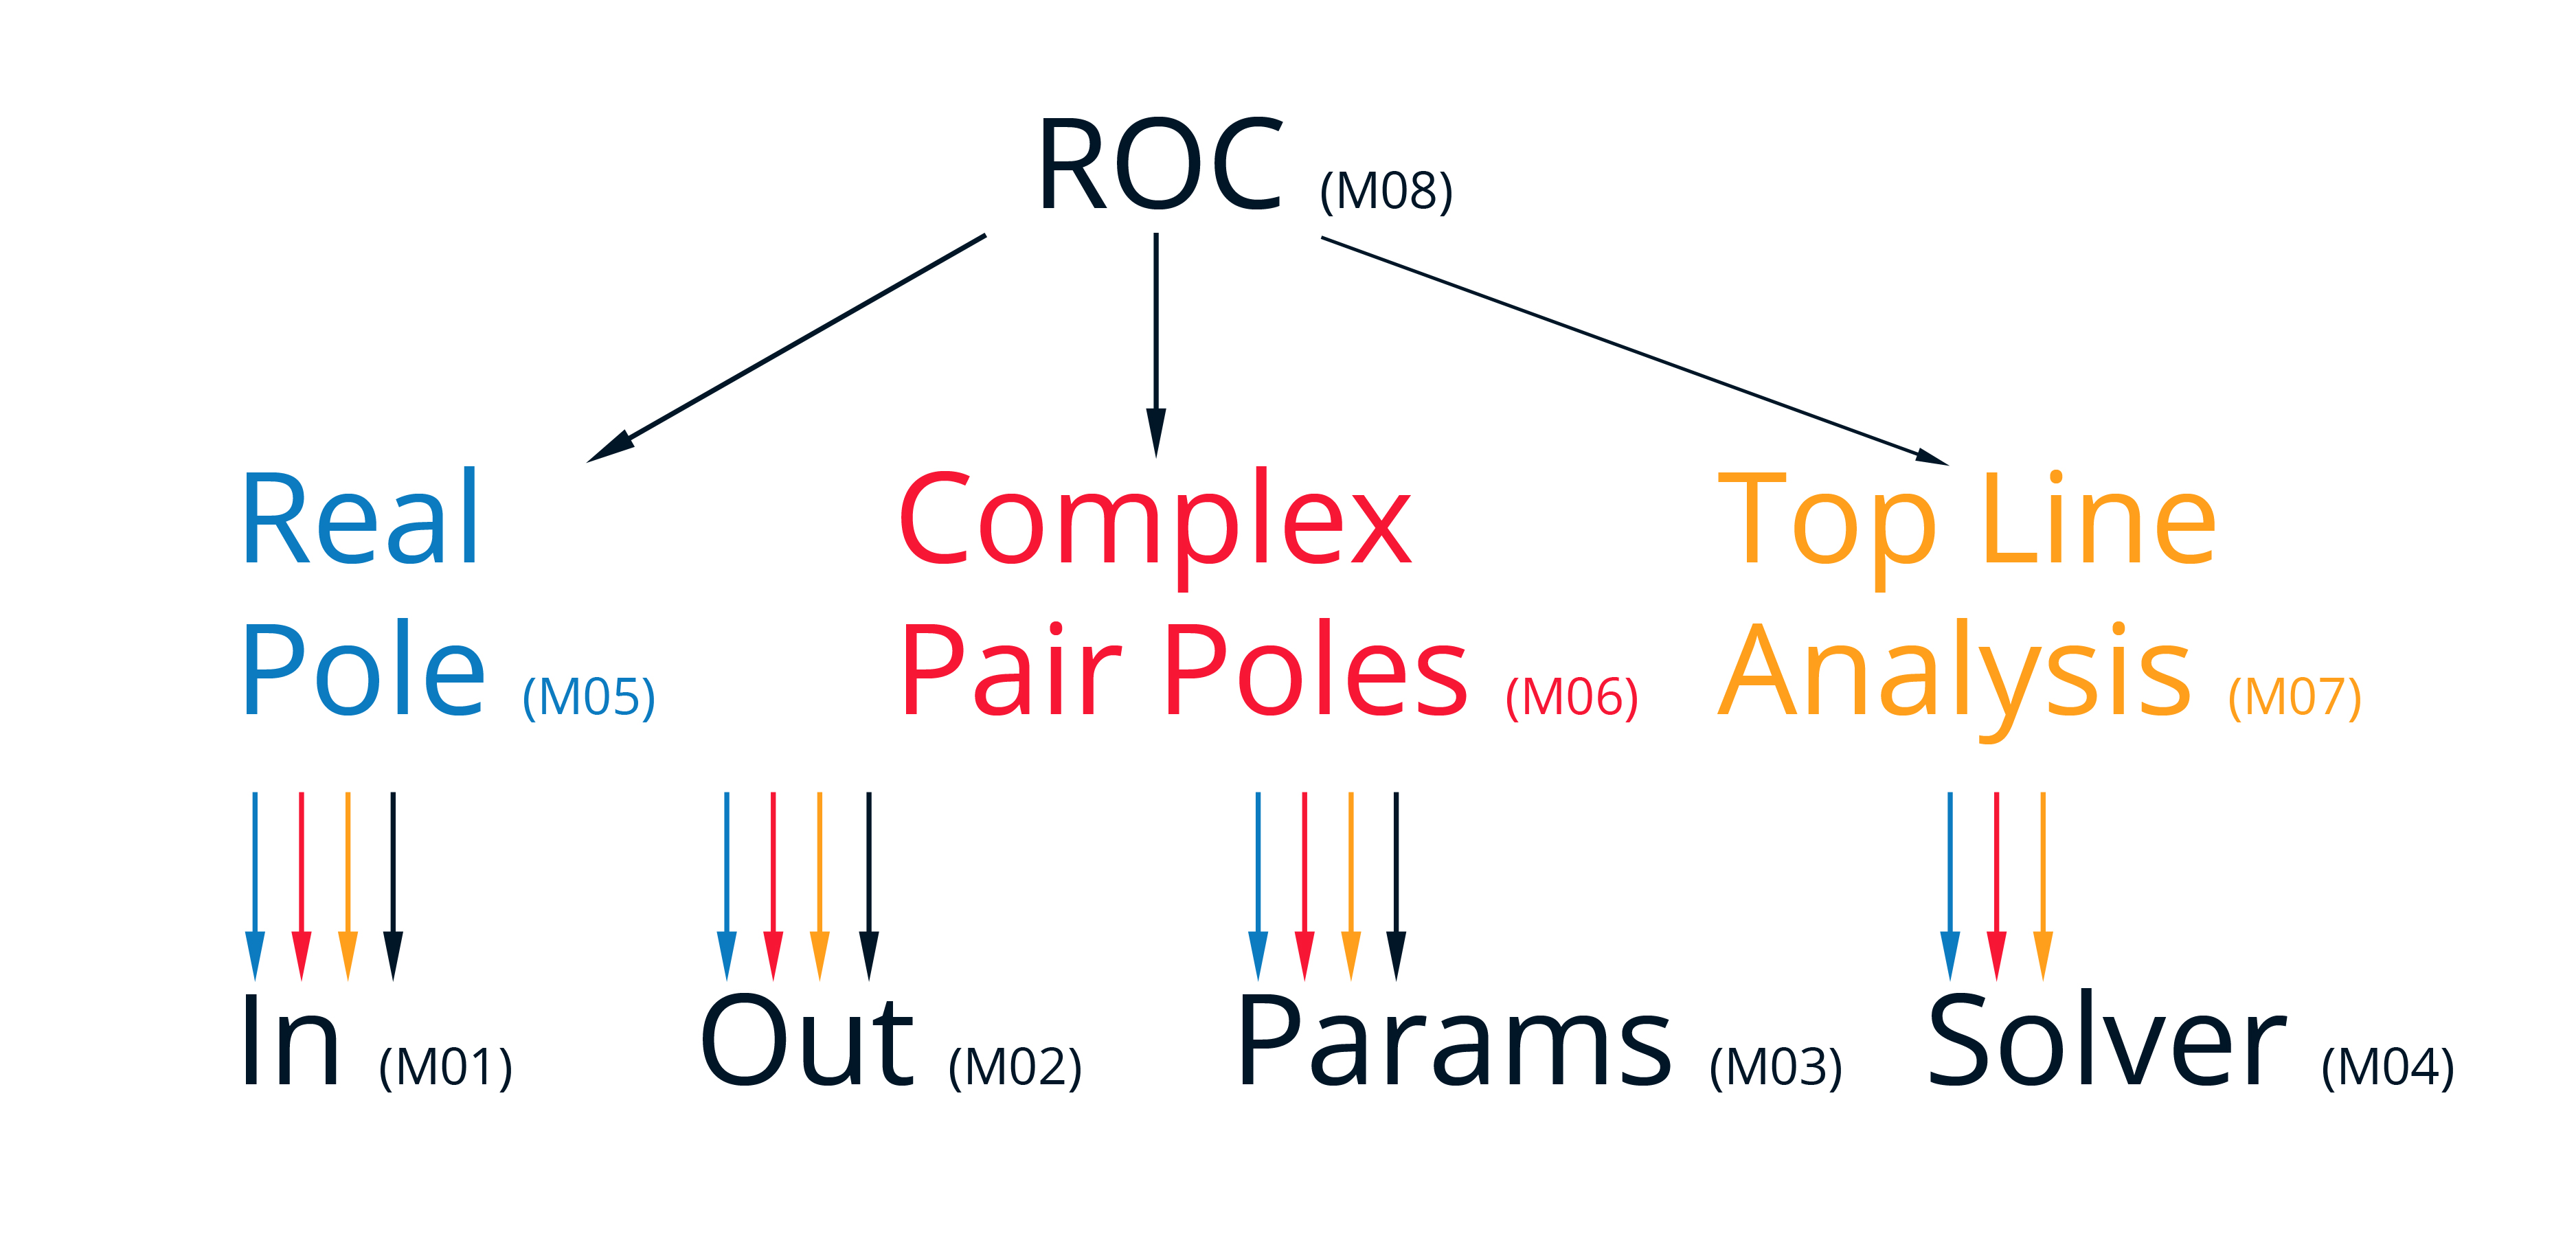
\includegraphics[width=0.9\textwidth]{roc-uses-diagram.jpg}
\caption{Use hierarchy among modules}
\label{FigUH}
\end{figure}

%\section*{References}

\bibliographystyle {plainnat}
\bibliography{../../refs/References}

\end{document}
